\let\negmedspace\undefined
\let\negthickspace\undefined
\documentclass[journal,12pt,onecolumn]{IEEEtran}
\usepackage{cite}
\usepackage{amsmath,amssymb,amsfonts,amsthm}
\usepackage{algorithmic}
\usepackage{graphicx}
\usepackage{textcomp}
\usepackage{xcolor}
\usepackage{txfonts}
\usepackage{listings}
\usepackage{enumitem}
\usepackage{mathtools}
\usepackage{gensymb}
\usepackage{comment}
\usepackage[breaklinks=true]{hyperref}
\usepackage{tkz-euclide} 
\usepackage{gvv}                                        
%\def\inputGnumericTable{}                                 
\usepackage[latin1]{inputenc}     
\usepackage{xparse}
\usepackage{color}                                            
\usepackage{array}                                            
\usepackage{longtable}                                       
\usepackage{calc}                                             
\usepackage{multirow}
\usepackage{multicol}
\usepackage{hhline}                                           
\usepackage{ifthen}                                           
\usepackage{lscape}
\usepackage{tabularx}
\usepackage{array}
\usepackage{float}
\newtheorem{theorem}{Theorem}[section]
\newtheorem{problem}{Problem}
\newtheorem{proposition}{Proposition}[section]
\newtheorem{lemma}{Lemma}[section]
\newtheorem{corollary}[theorem]{Corollary}
\newtheorem{example}{Example}[section]
\newtheorem{definition}[problem]{Definition}
\newcommand{\BEQA}{\begin{eqnarray}}
\newcommand{\EEQA}{\end{eqnarray}}
%\newcommand{\define}{\stackrel{\triangle}{=}}
\theoremstyle{remark}
%\newtheorem{rem}{Remark}
% Marks the beginning of the document
\begin{document}
\title{Architecture and Planning}
\author{AI25btech11027 - Bhuvana}
\maketitle
\renewcommand{\thefigure}{\theenumi}
\renewcommand{\thetable}{\theenumi}
\begin {center}
\textbf{Q1 to Q5 carry 1 mark each \&  Q6 to Q10 carry 2 marks each}

\end{center}

\begin{enumerate}


\item Choose the most appropriate word from the options given below to complete the following sentence:  

The principal presented the chief guest with a \underline{\makebox[2cm]{\hfill}}, as token of appreciation.\hfill \textbf{(GATE EE 2025)}
\begin{enumerate}
\begin{multicols}{4}
    \item Momento
    \item Memento  
    \item Momentum
    \item Moment
    \end{multicols}
\end{enumerate}


\item Choose the appropriate word/phrase, out of the four options given below, to complete the following sentence:  

Frogs \underline{\makebox[2cm]{\hfill}}.\hfill \textbf{(GATE EE 2025)}
\begin{enumerate}
\begin{multicols}{4}
    \item Croak
    \item Roar
    \item Hiss
    \item Patter
    \end{multicols}
\end{enumerate}


\item Choose the word most similar in meaning to the given word:  \\
Educe \hfill \textbf{(GATE EE 2025)}
\begin{enumerate}
\begin{multicols}{4}
    \item Exert
    \item Educate
    \item Extract 
    \item Extend
    \end{multicols}
\end{enumerate}


\item Operators $\Box$, $\diamondsuit$ and $\rightarrow$ are defined by:  \hfill \textbf{(GATE EE 2025)}
\begin{align}
a \Box b = \frac{a-b}{a+b}, \quad 
a \diamondsuit b = \frac{a+b}{a-b}, \quad 
a \rightarrow b = ab
\end{align}

Find the value of $(66 \Box 6) - (66 \diamondsuit 6)$.\hfill \textbf{(GATE EE 2025)}
\begin{enumerate}
\begin{multicols}{4}
    \item $-2$
    \item $-1$
    \item $1$ 
    \item $2$
    \end{multicols}
\end{enumerate}


\item If $\log_x \left(\frac{5}{7}\right) = -\frac{1}{3}$, then the value of $x$ is  \hfill \textbf{(GATE EE 2025)}
\begin{enumerate}
\begin{multicols}{4}
    \item $\frac{343}{125}$ \\
    \item $\frac{125}{343}$\\
    \item $-\frac{25}{49}$\\
    \item $-\frac{49}{25}$\\
    \end{multicols}
\end{enumerate}


\item The following question presents a sentence, part of which is underlined. Beneath the sentence you will find four ways of phrasing the underlined part. Following the requirements of the standard written English, select the answer that produces the most effective sentence.\\

Tuberculosis, together with its effects, \underline{ranks one of the leading causes of death in India}.\hfill \textbf{(GATE EE 2025)}
\begin{enumerate}
    \item ranks as one of the leading causes of death
    \item  rank as one of the leading causes of death
    \item has the rank of one of the leading causes of death
    \item are one of the leading causes of death
\end{enumerate}





\item Read the following paragraph and choose the correct statement.
\\
Climate change has reduced human security and threatened human well being. As an integral relation of human progress is that human security largely depends upon environmental security. But on the contrary, human progress seems contradictory to environmental security. To keep up both at the required level is a challenge to be addressed by one and all. One of the ways to curb the climate change may be suitable scientific innovations, while the other may be the Gandhian perspective of small scale progress with focus on sustainability.\hfill \textbf{(GATE EE 2025)}
\begin{enumerate}
    \item Human progress and security are positively associated with environmental security.
    \item Human progress is contradictory to environmental security.
    \item Human security is contradictory to environmental security.
    \item Human progress depends upon environmental security.
\end{enumerate}






\item Fill in the missing value.\hfill \textbf{(GATE EE 2025)}

\begin{figure}[h]
    \centering
    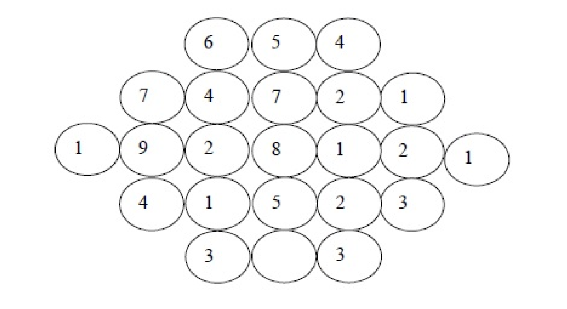
\includegraphics[width=0.5\linewidth]{figs/fig1.png}
    \caption{}
    \label{fig1}
\end{figure}


\item A cube of side 3 units is formed using a set of smaller cubes of side 1 unit. Find the proportion of the number of faces of the smaller cubes visible to those which are NOT visible.\hfill \textbf{(GATE EE 2025)}
\begin{enumerate}
\begin{multicols}{4}
    \item $1 : 4$
    \item $1 : 3$
    \item $1 : 2$
    \item $2 : 3$
    \end{multicols}
\end{enumerate}



\item Humpty Dumpty sits on a wall every day while having lunch. The wall sometimes breaks. A person sitting on the wall falls if the wall breaks.  \\
Which one of the statements below is logically valid and can be inferred from the above sentences?\hfill \textbf{(GATE EE 2025)}
\begin{enumerate}
    \item  Humpty Dumpty always falls while having lunch
    \item Humpty Dumpty does not fall sometimes while having lunch
    \item Humpty Dumpty never falls during dinner
    \item  When Humpty Dumpty does not sit on the wall, the wall does not break
\end{enumerate}

\begin{center}
    \textbf{Q11  to Q35 carry 1 mark each \& Q36 to Q65 carry 2 marks each}
\end{center}


\item  A Housing Finance Institution in the private sector is \hfill \textbf{(GATE EE 2025)} 
\begin{enumerate}
\begin{multicols}{4}
    \item HUDCO
    \item SBI
    \item PNB
    \item HDFC
    \end{multicols}
\end{enumerate}
\item  Which of the following statements regarding PERT is \textbf{NOT} true?  \hfill \textbf{(GATE EE 2025)}
\begin{enumerate}
    \item Each activity of PERT network has three different time estimates
    \item Expected activity time is estimated based on $\beta$-distribution
    \item PERT is a deterministic model
    \item PERT network may have more than one critical path
\end{enumerate}
\item Damage of foundation due to ``Soil Liquefaction'' is related to  \hfill \textbf{(GATE EE 2025)}
\begin{enumerate}
\begin{multicols}{4}
    \item Cyclones
    \item Landslides
    \item Floods
    \item Earthquakes
    \end{multicols}
\end{enumerate}
\item Walls with high thermal inertia are suitable in which type of climate?  \hfill \textbf{(GATE EE 2025)}
\begin{enumerate}
\begin{multicols}{4}
    \item Hot-dry
    \item Hot-humid
    \item Temperate
    \item Cold
    \end{multicols}
\end{enumerate}
\item The ratio of town area to agricultural land area as suggested by Sir Ebenezer Howard in ``Garden City'' concept is  \hfill \textbf{(GATE EE 2025)}
\begin{enumerate}
\begin{multicols}{4}
    \item $1:20$
    \item $1:15$
    \item $1:10$
    \item $1:5$
    \end{multicols}
\end{enumerate}
\item A ``Demolition Contract'' for a building is awarded to the \hfill \textbf{(GATE EE 2025)}  
\begin{enumerate}
\begin{multicols}{2}
    \item Lowest Bidder
    \item Highest Bidder
    \item Second Lowest Bidder
    \item Second Highest Bidder
    \end{multicols}
\end{enumerate}
\item Bulking of sand is highest in \hfill \textbf{(GATE EE 2025)} 
\begin{enumerate}
\begin{multicols}{2}
    \item Coarse sand
    \item Medium sand
    \item Fine sand
    \item Sand saturated with water
    \end{multicols}
\end{enumerate}

\item The Venice Charter (1964) led to the establishment of\hfill \textbf{(GATE EE 2025)}
\begin{enumerate}
    \item International Centre for the Study of the Preservation and Restoration of Cultural Property \brak{ICCROM}
    \item International Council on Monuments and Sites \brak{ICOMOS}
    \item Indian National Trust for Art and Cultural Heritage \brak{INTACH}
    \item Archaeological Survey of India \brak{ASI}
\end{enumerate}
\item The ratio between \textit{illumination at a working point indoor to total light available simultaneously outdoor} is known as\hfill \textbf{(GATE EE 2025)}
\begin{enumerate}
\begin{multicols}{2}
    \item Daylight Factor
    \item Sky Component
    \item Internally Reflected Component
    \item Externally Reflected Component
    \end{multicols}
\end{enumerate}
\item Which of the following vehicular traffic intersections converts all crossing into merging and diverging sequences?\hfill \textbf{(GATE EE 2025)}
\begin{enumerate}
\begin{multicols}{2}
    \item Rotary
    \item Manual Signaling
    \item Grade Separation
    \item Automatic Signaling
    \end{multicols}
\end{enumerate}
\item The process of spraying Polyester, Polyurethane, Acrylate and Epoxy Plastic, followed by heat curing onto metals is called\hfill \textbf{(GATE EE 2025)}
\begin{enumerate}
\begin{multicols}{2}
    \item Anodizing
    \item Galvanizing
    \item Vitreous Enameling
    \item Powder Coating
    \end{multicols}
\end{enumerate}
\item The fundamental right pertaining to property ownership in India \textbf{DOES NOT} embrace:\hfill \textbf{(GATE EE 2025)}
\begin{enumerate}
\begin{multicols}{2}
    \item Sell, Lease, Donate or Bequeath
    \item Mortgage
    \item Grant Easement
    \item Change in use
    \end{multicols}
\end{enumerate}

\item Match the \textbf{Elements} in Group I with their \textbf{Applications} in Group II. \hfill \textbf{(GATE EE 2025)}

\begin{tabular}{p{0.45\textwidth}p{0.45\textwidth}}
\textbf{Group I} & \textbf{Group II} \\
P. Bracket & 1. Door \\
Q. Baluster & 2. Dome \\
R. Keystone & 3. Cornice \\
S. Holdfast & 4. Arch \\
            & 5. Staircase \\
\end{tabular}
\begin{enumerate}
\begin{multicols}{2}
    \item P-2, Q-5, R-3, S-1
    \item P-3, Q-5, R-4, S-1
    \item P-3, Q-1, R-4, S-5
    \item P-2, Q-1, R-3, S-4
    \end{multicols}
\end{enumerate}
\item Match the \textbf{Buildings} in Group I with their \textbf{Principal Architects} in Group II.\\
\begin{tabular}{p{0.6\textwidth}p{0.45\textwidth}}
 P. Werner Centre for the Visual arts,Ohio    & 1. I.M.Pie \\
 Q. Vitra Fire station,Weilam Rhein,Germany    & 2. Peter Eisenman\\
 R. AT \& T Building, New York  &  3. Louis Kahn\\
 S. Sher-e-Banglanagar,Dacca  & 4. Zaha Hadid\\
          & 5. Philip Johnson\\
\end{tabular}
\begin{enumerate}
    \begin{multicols}{2}
        \item P-2,Q-4,R-5,S-3
        \item P-3,Q-5,R-4,S-1
        \item P-1,Q-2,R-5,S-3
        \item P-2,Q-4,R-1,S-5
    \end{multicols}
\end{enumerate}
\item  A combination of colours forming an equilateral triangle in a Colour Wheel is called
    \begin{enumerate}
    \begin{multicols}{2}
        \item Analogous Scheme
        \item Triad Scheme
        \item  Split Complementary Scheme
        \item  Double Complementary Scheme
        \end{multicols}
\end{enumerate}
\item  Desire Line diagram helps in
    \begin{enumerate}
        \item Completion of a project by a desired date
        \item Meeting demand and supply in desired category of housing
        \item Determining income versus expenditure pattern of individuals
        \item Origin-Destination analysis in transport planning
    \end{enumerate}
 \item  As per Fire Safety norms of NBC India for buildings having assembly and institutional occupancies, the maximum travel distance in meters to an exit from the dead end of a corridor is
    \begin{enumerate}
    \begin{multicols}{4}
        \item 30
        \item 24
        \item 12
        \item 6
        \end{multicols}
    \end{enumerate}
\item  Which of the following is a part of a studio apartment?
    \begin{enumerate}
        \item Master bed room
        \item Artist's room
        \item Multipurpose space
        \item Children's room
    \end{enumerate}
\item The Saturation level of a colour represents
    \begin{enumerate}
    \begin{multicols}{4}
        \item Distribution
        \item Brilliance
        \item Density
        \item Warmth
        \end{multicols}
    \end{enumerate}
\item Invert level of a pipe at a given cross section refers to the
\begin{enumerate}
    \begin{multicols}{2}
        \item highest point of the internal surface
        \item lowest point of the internal surface
        \item highest point of the external point
        \item lowest point of the internal point
    \end{multicols}
\end{enumerate}
\item The command DVIEW in AutoCAD permits to view
\begin{enumerate}
    \item a selected portion of the drawing in detail
    \item the entire screen on the monitor
    \item a perspective of the drawing
    \item a damaged part of the drawing
\end{enumerate}
\item Match the \textbf{Land use categories} of Group-I with their respective \textbf{Colour codes} in Group-II as per practice in India.\\
\begin{tabular}{p{0.45\textwidth}p{0.45\textwidth}}
P. Residential     & 1. Red \\
Q. Commercial     & 2. Grey\\
R. Industrial  &  3. Blue\\
S. Public / Semi-Public  &  4. Violet\\
   & 5. Yellow\\
\end{tabular}
\begin{enumerate}
\begin{multicols}{2}
    \item P-5,Q-3,R-4,S-1
    \item P-5,Q-4,R-2,S-1
    \item P-1,Q-2,R-4,S-5
    \item P-1,Q-3,R-2,S-4
    \end{multicols}
\end{enumerate}
\item A rectangular beam section of size $300\text{mm} \times 500\text{mm}$ (depth) is loaded with a shear force of $600\text{kN}$ .The maximum shear stress on the section in $N/mm^2$ is \underline{\makebox[2cm]{\hfill}}
\item In a $50\text{meter}$ section of a waste water pipe, if the gradient is 1 in 80 ,then the fall in millimeter is \underline{\makebox[2cm]{\hfill}}
\item A $15\text{meter}$ long $3\text{meter}$ wide driveway needs to be paved with $300\text{mm} \times 300\text{mm}$ square tiles. If each packet contains 30 number of tiles,then the number of packets to be procured to pave the 
\item Match the \textbf{Monuments} in Group I with their \textbf{Features} in Group II. \hfill \textbf{(GATE EE 2025)}
\begin{tabular}{p{0.5\textwidth}p{0.5\textwidth}}
Group I  & Group II \\
P. Panch Mahal,Fathepur sikri     & 1. Painted Stone Figures \\
Q. Meenakshi Temple,Madhurai     & 2. Intricate Red Sand Stone Carvings\\
R. Jor-Bangla Temple,Bishnupur  & 3. Granite Statues\\
S. Sun Temples,Konark     & 4. Khondalite Stone Work\\
     & 5. Terracotta Carvings\\
\end{tabular}
\begin{enumerate}
\begin{multicols}{2}
\item P-2,Q-1,R-4,S-3
\item P-2,Q-1,R-5,S-4
\item P-2,Q-4,R-1,S-3
\item P-1,Q-5,R-5,S-4
\end{multicols}
\end{enumerate}
\item Match the \textbf{Monuments} in Group I with their \textbf{Style of Architecture} in Group II \hfill \textbf{(GATE EE 2025)}
\begin{tabular}{p{0.5\textwidth}p{0.5\textwidth}}
P. Pisa Cathedral,Italy     & 1. Gothic \\
Q. St.Hagia Sophia,Isthanbul     & 2. Moorish\\
R. Great Temple of Aman,Karnak & 3. Egyptian\\
S. Cathedral of Notre Dame,Paris & 4. Byzantine\\
    & 5. Romanesque\\
    \begin{enumerate}
        \begin{multicols}{2}
            \item P-5,Q-1,R-3,S-2
            \item P-2,Q-4,R-3,S-5
            \item P-4,Q-2,R-5,S-1
            \item P-5,Q-4,R-3,S-1
        \end{multicols}
    \end{enumerate}
\end{tabular}
\item Match the \textbf{Buildings} in Group I with their \textbf{style of Architecture} in Group II. \hfill \textbf{(GATE EE 2025)}
\begin{tabular}{p{0.6\textwidth}p{0.45\textwidth}}
Group I  &  Group II \\
P. Rashtrapathi Bhawan,New Delhi     & 1. Industrial Architecture \\
Q. German Pavilion for World Exhibition,Barcelona     & 2. Deconstruction\\
R. Guggenheim Museum,Bilbao  & 3. Radical Eclecticism\\
S. Cathedral of Notre Dame,Paris  & 4. Byzantine\\
     & 5. Romanesque\\
\end{tabular}
\begin{enumerate}
    \begin{multicols}{2}
        \item P-5,Q-3,R-2,S-1
        \item P-5,Q-4,R-2,S-1
        \item P-1,Q-5,R-4,S-3
        \item P-3,Q-4,R-1,S-5
    \end{multicols}
\end{enumerate}
\item Match the \textbf{Terms} in Group I with their \textbf{Definitions} in Group II. \hfill \textbf{(GATE EE 2025)}
\begin{tabular}{p{0.4\textwidth}p{0.6\textwidth}}
P. Kinesthesia     & 1. Measurement and study of size and propositions of human body \\
Q. Anthropometry     & 2. Study of man-machine interaction\\
R. Ergonomics  & 3. Study of past and present of the human race\\
S. Biomimicry  & 4. Study of human sensory experience during movement\\
      & 5. Imitation of models,system and elements of nature\\
\end{tabular}
\begin{enumerate}
    \begin{multicols}{2}
        \item P-5,Q-3,R-4,S-1
        \item P-5,Q-2,R-4,S-3
        \item P-4,Q-1,R-2,S-5
        \item P-4,Q-1,R-2,S-3
    \end{multicols}
\end{enumerate}
\item Match the following \textbf{Urban Spaces} in Group I with their \textbf{Names} in Group II. \hfill \textbf{(GATE EE 2025)}
\begin{figure}[H]
    \centering
    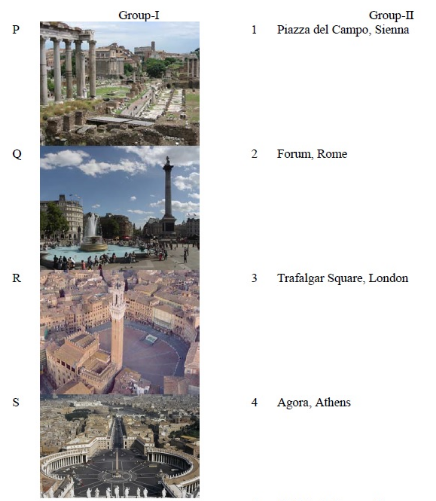
\includegraphics[width=0.5\linewidth]{figs/fig2.png}
    \caption{}
    \label{fig2}
\end{figure}
\begin{enumerate}
    \begin{multicols}{2}
        \item P-4,Q-1,R-2,S-3
        \item P-2,Q-3,R-1,S-5
        \item P-4,Q-3,R-1,S-5
        \item P-2,Q-1,R-4,S-3
    \end{multicols}
\end{enumerate}
\item Match the \textbf{Terms} in Group I with the appropriate \textbf{Items} in Group II.\hfill \textbf{(GATE EE 2025)}\\
\begin{tabular}{p{0.45\textwidth}p{0.45\textwidth}}
\textbf{Group I}  & \textbf{Group II}\\
P. Toposheet     & 1. Path/Row \\
Q. Satellite Image     & 2. Contour\\
R. Wavelength   & 3. Focal Length\\
S. Scan Line   & 4. Spectral Signature\\
            & 5. Bits/inch\\
\end{tabular}
\begin{enumerate}
    \begin{multicols}{2}
        \item P-5,Q-4,R-2,S-1
        \item P-5,Q-1,R-4,S-3
        \item P-2,Q-1,R-4,S-5
        \item P-2,Q-4,R-1,S-5
    \end{multicols}
\end{enumerate}
\item Match the \textbf{Concepts} in Group I with their appropriate \textbf{Explanation} in Group II.\hfill \textbf{(GATE EE 2025)}\\
\begin{tabular}{p{0.4\textwidth}p{0.6\textwidth}}
\textbf{Group I}  & \textbf{Group II}\\
P. Planned Unit Development     & 1.Development occuring on vacant or underused lots in otherwise built up areas \\
Q. Infill Development     & 2. Development providing a fair and equitable way to integrate peri-urban areas\\
R. Transit Oriented Development  & 3. Developing a large area as a single entity merging zoning and subdivision control\\
S. Mixed Use Development & 4. Development with compatible land uses integrating varied activities at different times of day\\
     & 5. Development located within walking distance from mass transit stations along the corridor\\
\end{tabular}
\begin{enumerate}
    \begin{multicols}{2}
        \item P-3,Q-2,R-5,S-4
        \item P-3,Q-1,R-5,S-4
        \item P-2,Q-1,R-4,S-5
        \item P-2,Q-4,R-1,S-5
    \end{multicols} 
\end{enumerate}
\item Particles of soil in \textbf{descending order} of grain size is
\begin{enumerate}
    \begin{multicols}{2}
        \item Gravel-Sand-Silt-Clay
        \item Gravel-Sand-Clay-Silt
        \item Sand-Gravel-Clay-Silt
        \item Clay-Gravel-Sand-Silt
    \end{multicols}
\end{enumerate}
\item Match the \textbf{Units} in Group I with their \textbf{Definition} in Group II.\hfill \textbf{(GATE EE 2025)}\\
\begin{tabular}{p{0.45\textwidth}p{0.5\textwidth}}
\textbf{Group I} & \textbf{Group II}\\
P. Hertz     & 1. Newton-meter \\
Q. Lux     & 2. $Cycles/second$ \\
R. Joule   & 3. $Lumen/m^2$ \\
S. Newton  & 4. $Watt/ampere$ \\
         & 5. kg-$meter/sec^2$\\
\end{tabular}
\begin{enumerate}
    \begin{multicols}{2}
        \item P-5,Q-4,R-2,S-1
        \item P-3,Q-1,R-5,S-4
        \item P-2,Q-3,R-1,S-4
        \item P-2,Q-3,R-1,S-5
    \end{multicols}
\end{enumerate}
\item Match the \textbf{Energy Efficient Building Elements} in Group I with their associated \textbf{Working Principles} in Group II.\hfill \textbf{(GATE EE 2025)}
\begin{tabular}{p{0.45\textwidth}p{0.45\textwidth}}
\textbf{Group I}     & \textbf{Group II}  \\
P. Solar Chimney     & 1. Thermal Storage\\
Q. Earth Air Tunnel & 2. Radiant Cooling\\
R. Trombe Wall  & 3. Stack Effect\\
S. Chilled Slab  & 4. Cross Ventilation\\
         & 5. Geothermal Energy\\
\end{tabular}
\begin{enumerate}
    \begin{multicols}{2}
        \item P-3,Q-2,R-4,S-5
        \item P-5,Q-2,R-4,S-3
        \item P-3,Q-5,R-1,S-2
        \item P-4,Q-5,R-1,S-2
    \end{multicols}
\end{enumerate}
\item Match the \textbf{Vibrator Types} in Group I with their related \textbf{Areas of Application} in Group II.\hfill \textbf{(GATE EE 2025)}\\
\begin{tabular}{p{0.45\textwidth}p{0.45\textwidth}}
\textbf{Group I} & \textbf{Group II}\\
P. Needle Vibrator     &1. Concrete Pavement  \\
Q. Shutter Vibrator     &2. Pre-cast Concrete Unit\\
R. Surface Vibrator    & 3. Beam-Column Junction\\
S. Table Vibrator   & 4. Retaining Wall\\
     & 5. Slip Forming\\
\end{tabular}
\begin{enumerate}
    \begin{multicols}{2}
        \item P-1,Q-5,R-4,S-3
        \item P-3,Q-4,R-1,S-2
        \item P-1,Q-4,R-2,S-5
        \item P-3,Q-5,R-1,S-2
    \end{multicols}
\end{enumerate}
\item Match the type of \textbf{Temporary Structures} in Group I with their corresponding \textbf{Functions} in Group II.\hfill \textbf{(GATE EE 2025)}
\begin{tabular}{p{0.4\textwidth}p{0.6\textwidth}}
\textbf{Group I} & \textbf{Group II} \\
P. Scaffolding     &1. To support unsafe structure  \\
Q. Formwork     &2. To support platforms for workmen and materials at raised height during constuction\\
R. Shoring    & 3. Removal of water from pits\\
S. Underpinning & 4. Mould for RCC structure\\
     & 5. Strengthening the existing foundation\\
\end{tabular}
\begin{enumerate}
    \begin{multicols}{2}
        \item P-2,Q-4,R-1,S-5
        \item P-3,Q-5,R-1,S-2
        \item P-3,Q-4,R-5,S-2
        \item P-2,Q-3,R-4,S-5
    \end{multicols}
\end{enumerate}
\item Match the following \textbf{Scientific Names} in Group I with their common \textbf{Indian Names} in Group II.\hfill \textbf{(GATE EE 2025)}
\begin{tabular}{p{0.5\textwidth}p{0.5\textwidth}}
Group I & Group II\\
P. Lagerstroemia speciosa     &1. Amaltas  \\
Q. Cassia fistula     & 2. Neem\\
R. Azadarachta indica & 3. Jarul\\
S. Acacia auriculiformis & 4. Babul\\
       & 5. peepal\\
\end{tabular}
\begin{enumerate}
    \begin{multicols}{2}
        \item P-2,Q-4,R-3,S-5
        \item P-5,Q-3,R-2,S-4
        \item P-3,Q-1,R-4,S-2
        \item P-3,Q-1,R-2,S-4
    \end{multicols}
\end{enumerate}
\item A man starts from his residence and uses the following modes in sequence to reach his office by cycle rickshaw to railway station,then train to destination station,followed by auto-rickshaw to nearby bus stand and finally a bus to his office.Which of the following describes his sequence of transit usage ?
\begin{enumerate}
    \item Non Motorised Transit-Paratransit-Mass Transit-Public Transit
    \item Paratransit-Public Transit-Non Motorised Transit-Mass Transit
    \item Private Transit-Public Transit-Non Motorised Transit-Mass Transit
    \item Non Motorised Transit-Mass Transit-Paratransit-Public Transit
\end{enumerate}
\item PMGSY and JNNURM are two Indian Government programmes which  deal with
\begin{enumerate}
    \item rural road development and urban basic service improvement respectively
    \item rural sanitation service and under-developed road maintenance respectively
    \item peri-urban basic services and urban basic service improvement respectively
    \item rural road development and urbans transport development respectively
\end{enumerate}
\item Match the \textbf{Planning Terms} in Group I with their \textbf{Descriptions} in Group II.\hfill \textbf{(GATE EE 2025)}
\begin{tabular}{p{0.45\textwidth}p{0.6\textwidth}}
P. Gentrification     &1. Haphazard and low density outward growth of urban area  \\
Q. Urban core revitalization     &2. Primarily dormitory settlement with functional dependency on parent city\\
R. Urban sprawl   & 3. Replacement of low income residents with high income population\\
S. Satellite town & 4. Physical and socio-economic revival of the inner-city\\
       & 5. Restricted development in an environmentally sensitive zone\\
\end{tabular}
\begin{enumerate}
    \begin{multicols}{2}
        \item P-4,Q-3,R-5,S-2
        \item P-3,Q-4,R-1,S-2
        \item P-1,Q-5,R-2,S-3
        \item P-3,Q-4,R-1,S-2
    \end{multicols}
\end{enumerate}
\item Match the \textbf{Planning Concepts} in Group I with their \textbf{Corresponding proponents} in Group II.\hfill \textbf{(GATE EE 2025)}
\begin{tabular}{p{0.45\textwidth}p{0.45\textwidth}}
Group I  & Group II\\
P. Broadacre city     &1. Le Corbusier  \\
Q. Radiant city     & 2. F.L.Wright\\
R. Industrial town & 3. Robert Owen\\
S. Acrosanti  & 4. Henry Wright\\
    & 5. Paolo Soleri\\
\end{tabular}
\begin{enumerate}
    \begin{multicols}{2}
        \item P-1,Q-4,R-3,S-5
        \item P-1,Q-3,R-5,S-2
        \item P-2,Q-1,R-3,S-5
        \item P-2,Q-1,R-5,S-4
    \end{multicols}
\end{enumerate}
\item The housing stock of a town has total number of $9090$ dwelling units.Present population of the town is $45,450$.Assuming an average household size of $4.5$,the housing shortage in percentage is \underline{\makebox[2cm]{\hfill}} \hfill \textbf{(GATE EE 2025)}
\item A hall is $15$ m long and $12$ m wide.If the sum of areas of the floor and cieling is equal to the sum of the area of its four walls,then the volume of the hall in cubic meter is \underline{\makebox[2cm]{\hfill}} \hfill \textbf{(GATE EE 2025)}
\item The actual roof area of a building is $3,60,000\text{sqm}$ which on a site plan measures $25\text{sqcm}$ The scale of the site plan is 1:\underline{\makebox[2cm]{\hfill}} \hfill \textbf{(GATE EE 2025)}
\item If the annual net income from the commercial property is Rs $22,000$/- and the interest is $8\%$ then the capitalized value in rupees of the property in perpetuality is \underline{\makebox[2cm]{\hfill}} \hfill \textbf{(GATE EE 2025)}
\item A five storied building is constucted on a $100\text{m} \times 50\text{m}$ plot having ground coverage of $60\%$ (option 1).Alternatively ,a four storied building is constructed on the same plot with a $50\%$ ground coverage (option 2).The ratio of FARs between options 1 and 2 is \underline{\makebox[2cm]{\hfill}} \hfill \textbf{(GATE EE 2025)}
\item If a roof is treated with a layer of thermal insultation material ,the internal heat gain is reduced by $60\%$ The U-value of the roof slab (without thermal insultation) is $3 Wm^2/$$^\circ{C}$  Assuming a constant temparature difference between indoor the U-value of the thermal insulation layer in $Wm^2/$$^\circ{C}$ is \underline{\makebox[2cm]{\hfill}} \hfill \textbf{(GATE EE 2025)}
\item A simply supported beam having effective span of $5\text{meter}$ is carrying a centrally concentrated load of $16\text{kN}$.The maximum bending moment in the beam in kN-m is \underline{\makebox[2cm]{\hfill}} \hfill \textbf{(GATE EE 2025)}
\item A landscaped garden with irregular profile and minor undulations,measuring $35,000\text{sqm}$ has a totl surface area covered with $20\%$ brick paving,$15\%$ cement concrete paving,and rest with grass.The peak intensity of rainfall in tht region is $70 mm/hr$.The coefficient of runoff for brick paving, cement concrete paving and grass is $0.8,0.9$ and $0.5$ respectively.The estimated quantity of runoff in $cubic meter/hr$ for the entire garden area is \underline{\makebox[2cm]{\hfill}} \hfill \textbf{(GATE EE 2025)}
\item The number of standard cement bags required to prepare $1400\text{kg}$ of concrete in the ratio $1:2:4$ (mixed by weight batching) is \underline{\makebox[2cm]{\hfill}} \hfill \textbf{(GATE EE 2025)}
\item A classroom measuring $10\text{m} \quad (L) \times 8\text{m} \quad (B) \times 2.7\text{m} \quad (H)$ requires an illumination level of $500$ lux on the desk level using $40\text{W}$ fluorescent lamps with rated output of $5000$ lumens each.Assuming utilization factor of $0.5$ and the maintenance factor of $0.8$, the number of lamps required is \underline{\makebox[2cm]{\hfill}} \hfill \textbf{(GATE EE 2025)}
\item Area of tensile steel per meter width of a reinforced concrete slab is $355\text{sq mm}$. If $8\text{mm}$ rods are used as reinforcement,then centre to centre spacing of the reinforcement in mm is \underline{\makebox[2cm]{\hfill}} \hfill \textbf{(GATE EE 2025)}
\item The population of a town as per census 2011 was $22,730$ and the population as per census 2001 was $15,770$.Considering arithmetic projection of growth,the projected population in 2016 will be \underline{\makebox[2cm]{\hfill}} \hfill \textbf{(GATE EE 2025)}
\item Two concrete mixers of capacity $200\text{litres}$ each are used in a construction site to produce $20 \text{cubic meter}$ of concrete .Ingredient charging ,mixing and discharge times are 3 minutes ,7 minutes and 1 minute respectively.Assuming a time loss of 5 minutes per hour of operation, the total time in hours for the mixers to produce the required amount of concrete will be \underline{\makebox[2cm]{\hfill}} \hfill \textbf{(GATE EE 2025)}
\end{enumerate}

   
   \end{document}
